\hsection{Entity Relationship Diagrams}%
We now know that entity types with their attributes basically correspond to datastructures in programming.
They form one element of the conceptual model.
But how do we actually write them down?
How do we specify them?

For this, a graphical notation has been introduced:
\glsreset{ERD}\Pglspl{ERD} are the most commonly used tool to model the entity types and their relationships in a \db~\cite{C2002ERMHEFTALL,C1975TRMTAUVOD,C1976TERMTAUVOD,KW2012ASHOTEDAIM,WF1995DHQDM,B1990CMERMO}.
There exists a wide variety of graphical notations that can be used for \pglspl{ERD}.
The original notations by \citeauthor{B1969DSD}~\cite{B1969DSD} and \citeauthor{C1975TRMTAUVOD}~\cite{C1975TRMTAUVOD,C1976TERMTAUVOD} are still in use, the more comprehensive and standardized \pgls{IDEF1X} syntax~\cite{FIPSPUB184,ISOIECIEEE2012ITMLP2SASFII}, and the \glsreset{UML}\pgls{UML}~\cite{OMG2017OUMLOU,RMHOSMUUIIIIOPPTRS1997UNG,BRJ1999TUMLRM}.
Indeed, there are many different flavors of diagrams that can serve as \pglspl{ERD}.
\Citeauthor{S2024D:CDMERDE}~\cite{S2024D:CDMERDE}, for example, presents nine slightly different variations.
\Citeauthor{SS2005EIDDDFDB:CDDRAAML}~\cite{SS2005EIDDDFDB:CDDRAAML} has two baseline variants, including several slight variations of a \pgls{UML}-based approach~(which is not listed in~\cite{S2024D:CDMERDE}).
The notation used by \citeauthor{V1999C5DMS:CDUTERM}~\cite{V1999C5DMS:CDUTERM} is yet again slightly different.

Honestly, I think the notation does not matter too much, as long as it is used consistently.%
%
\begin{figure}%
\centering%
%
\subfloat[][%
We open the \yEd\ editor and click on the \menu{Entity Relationship} tab in the \menu{Palette} view on the right-hand side.%
\label{fig:yedErdEntitiesA01scrollToErd}%
]{\tightbox{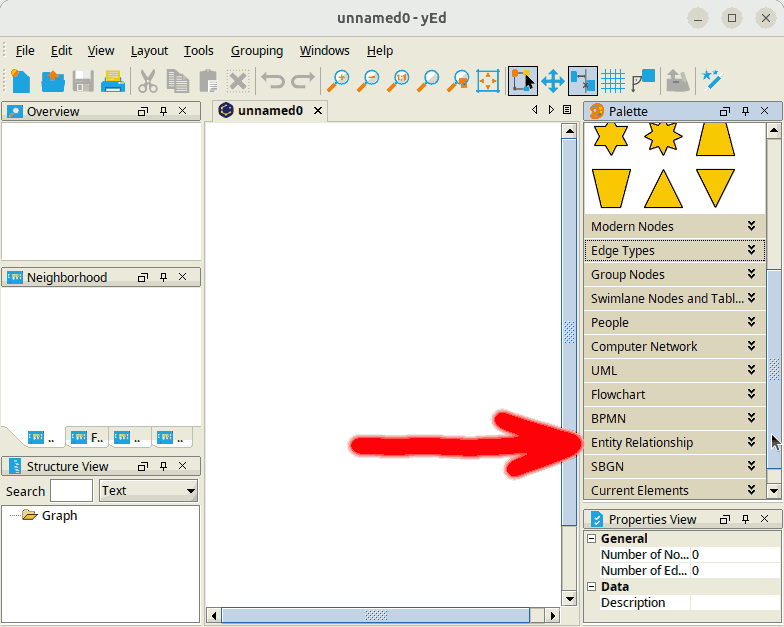
\includegraphics[width=0.48\linewidth]{\currentDir/yedErdEntitiesA01scrollToErd}}}%
%
\floatSep%
%
\subfloat[][%
We can now click on the \menu{Entity} symbol and drag it into the empty document.%
\label{fig:yedErdEntitiesA02entity}%
]{\tightbox{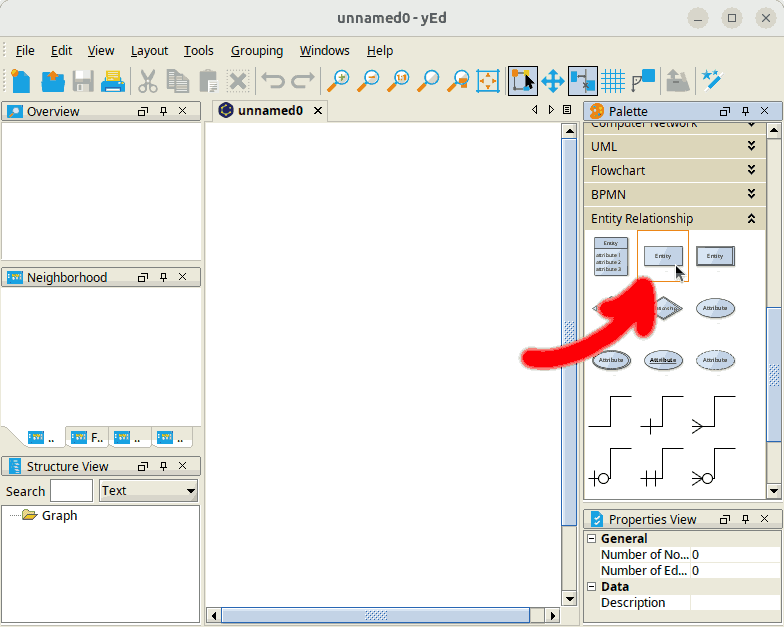
\includegraphics[width=0.48\linewidth]{\currentDir/yedErdEntitiesA02entity}}}%
%
\floatRowSep
%
\subfloat[][%
We dragged the entity symbol into the diagram document.%
\label{fig:yedErdEntitiesA03dragEntity}%
]{\tightbox{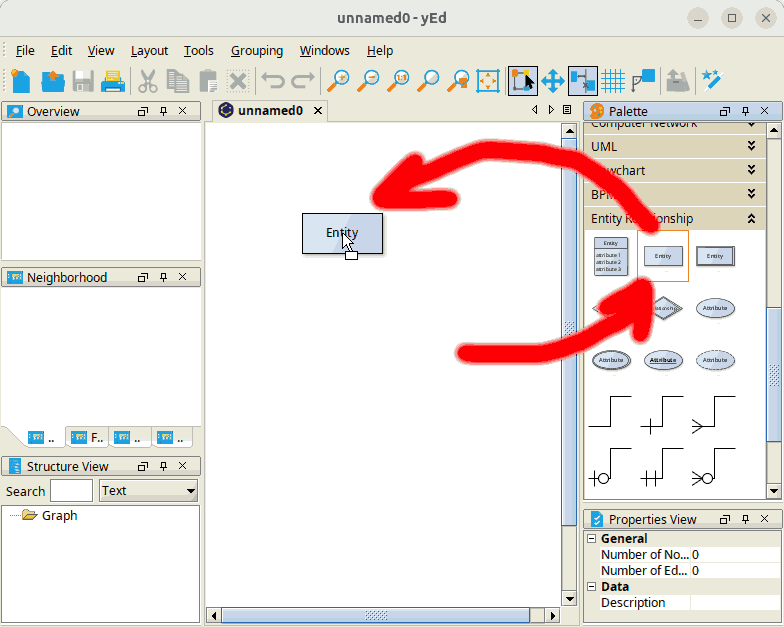
\includegraphics[width=0.48\linewidth]{\currentDir/yedErdEntitiesA03dragEntity}}}%
%
\floatSep
%
\subfloat[][%
We double-click into the new entity symbol in order to edit its name.%
\label{fig:yedErdEntitiesA04doubleClickName}%
]{\tightbox{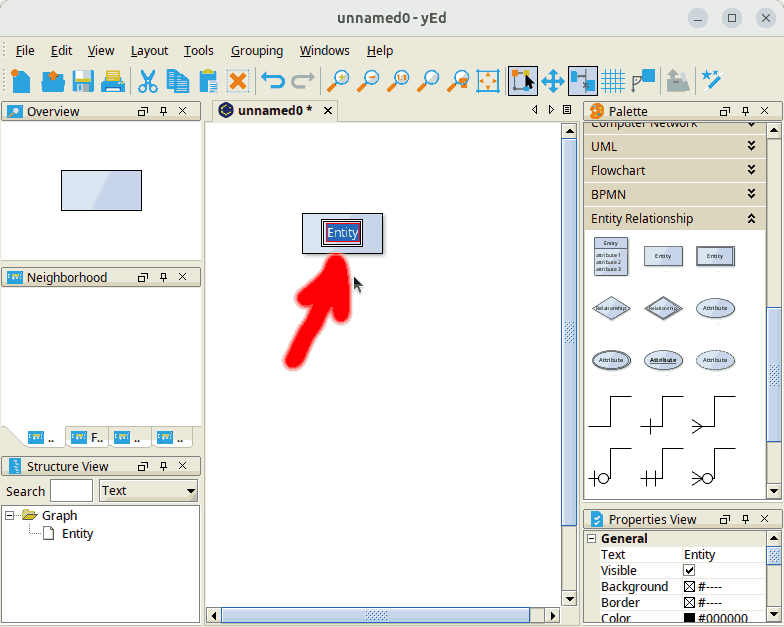
\includegraphics[width=0.48\linewidth]{\currentDir/yedErdEntitiesA04doubleClickName}}}%
%
\floatRowSep
%
\subfloat[][%
We change the entity name to \inQuotes{Student} and press \keys{\enter}.%
\label{fig:yedErdEntitiesA05changeNameToStudent}%
]{\tightbox{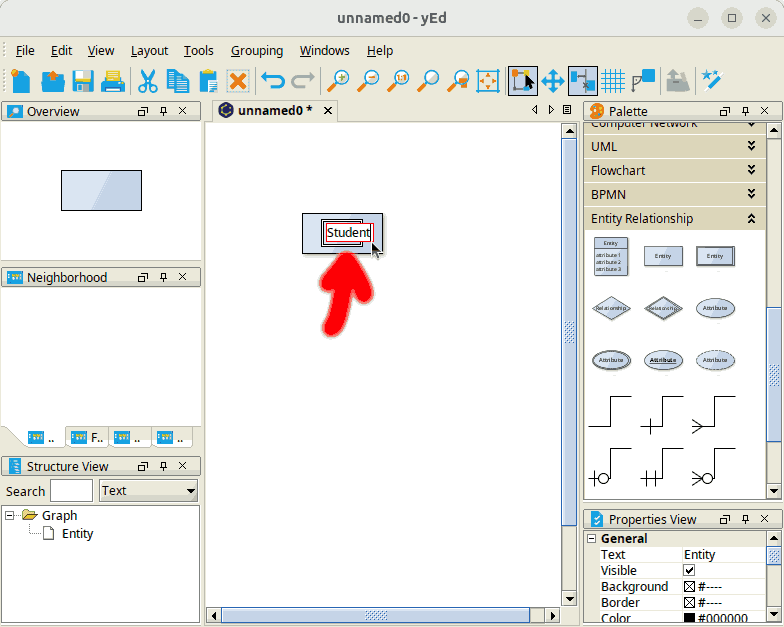
\includegraphics[width=0.48\linewidth]{\currentDir/yedErdEntitiesA05changeNameToStudent}}}%
%
\floatSep
%
\subfloat[][%
The name has changed. We now click on the \menu{Attribute} symbol in the element palette.%
\label{fig:yedErdEntitiesA06nameIsStudentSelectAttribute}%
]{\tightbox{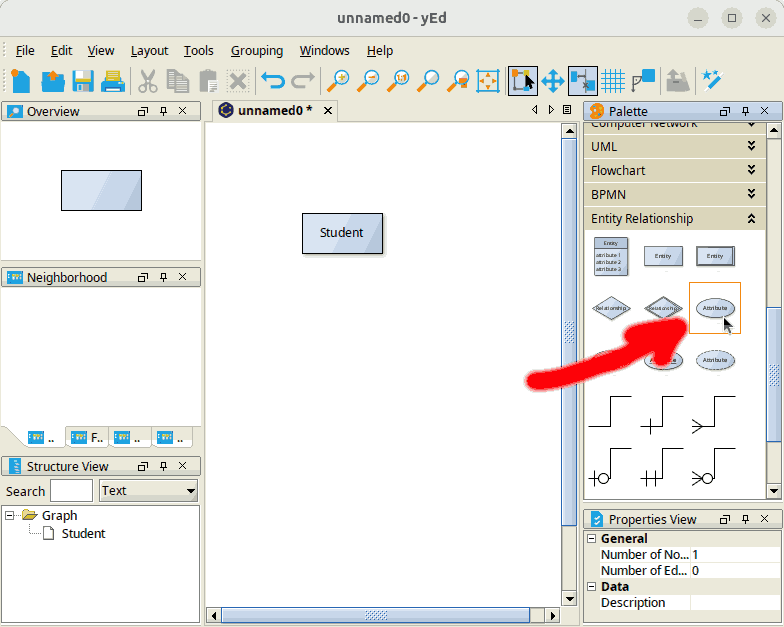
\includegraphics[width=0.48\linewidth]{\currentDir/yedErdEntitiesA06nameIsStudentSelectAttribute}}}%
%
\caption{Drawing an \pgls{ERD} with the \emph{Student} entity.}%
\label{fig:yedErdEntitiesA:A}%
\end{figure}%
%
\begin{figure}%
\ContinuedFloat%
\centering%
%
\subfloat[][%
We drag the attribute symbol into our document.%
\label{fig:yedErdEntitiesA07dragAttribute}%
]{\tightbox{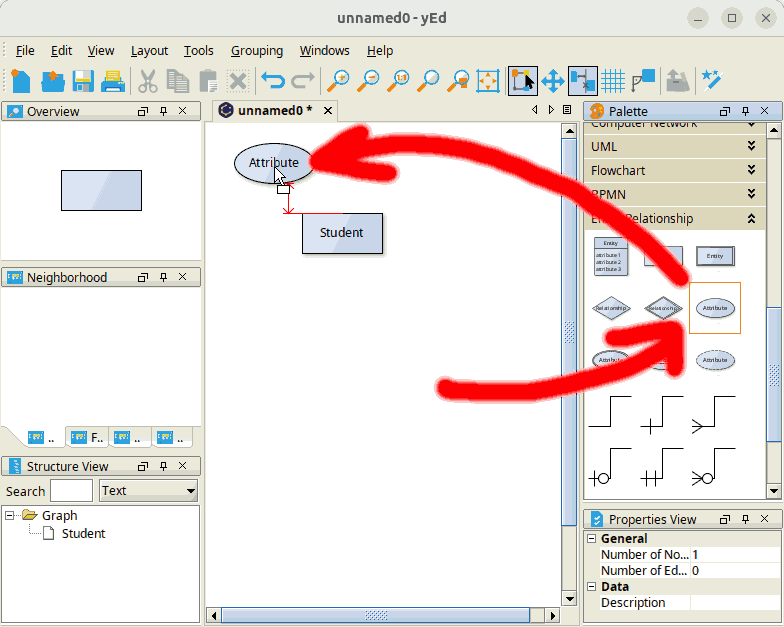
\includegraphics[width=0.48\linewidth]{\currentDir/yedErdEntitiesA07dragAttribute}}}%
%
\floatSep%
%
\subfloat[][%
We double-click into it to change its name.%
\label{fig:yedErdEntitiesA08doubleClickName}%
]{\tightbox{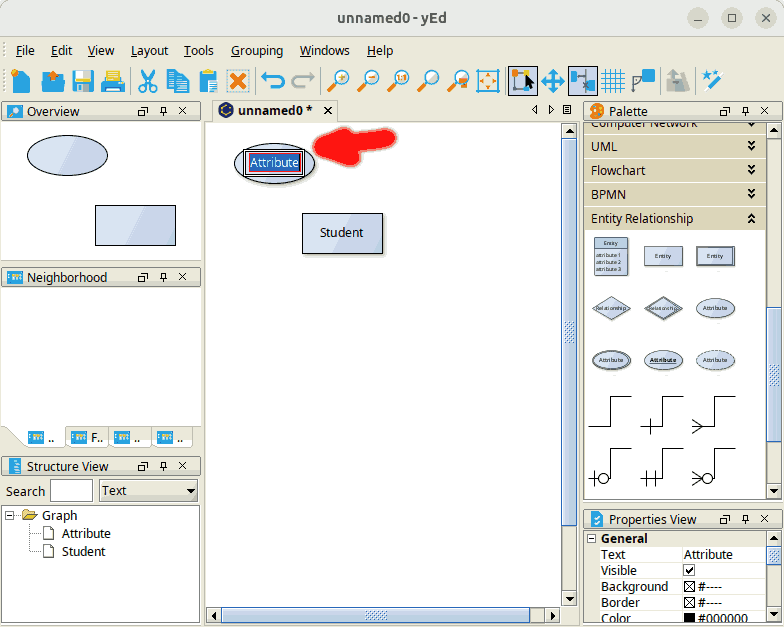
\includegraphics[width=0.48\linewidth]{\currentDir/yedErdEntitiesA08doubleClickName}}}%
%
\floatRowSep
%
\subfloat[][%
We want its name to be, well, \inQuotes{Name.}%
\label{fig:yedErdEntitiesA09changeNameToName}%
]{\tightbox{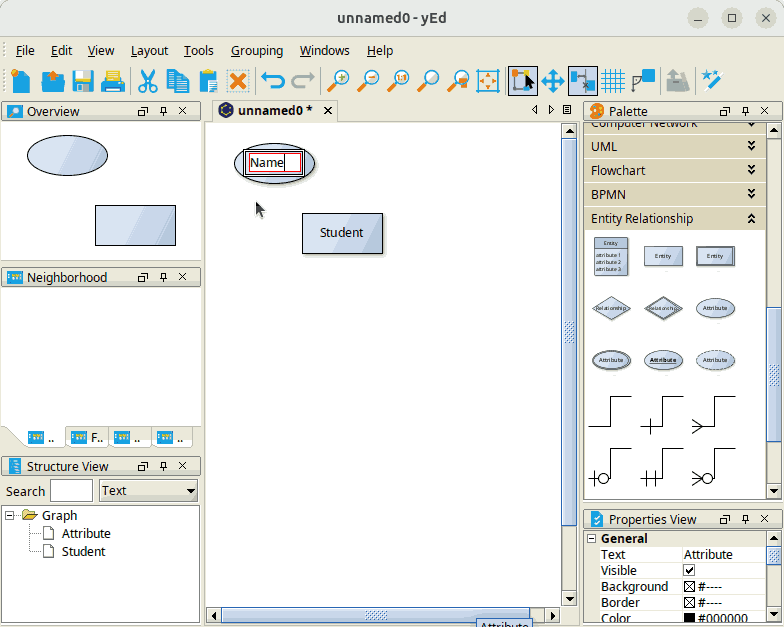
\includegraphics[width=0.48\linewidth]{\currentDir/yedErdEntitiesA09changeNameToName}}}%
%
\floatSep
%
\subfloat[][%
We changed the attribute name. %
Now we click on the connection symbol in the palette and drag it right onto the attribute.%
\label{fig:yedErdEntitiesA10changeNameChangedToNameSelectConnection}%
]{\tightbox{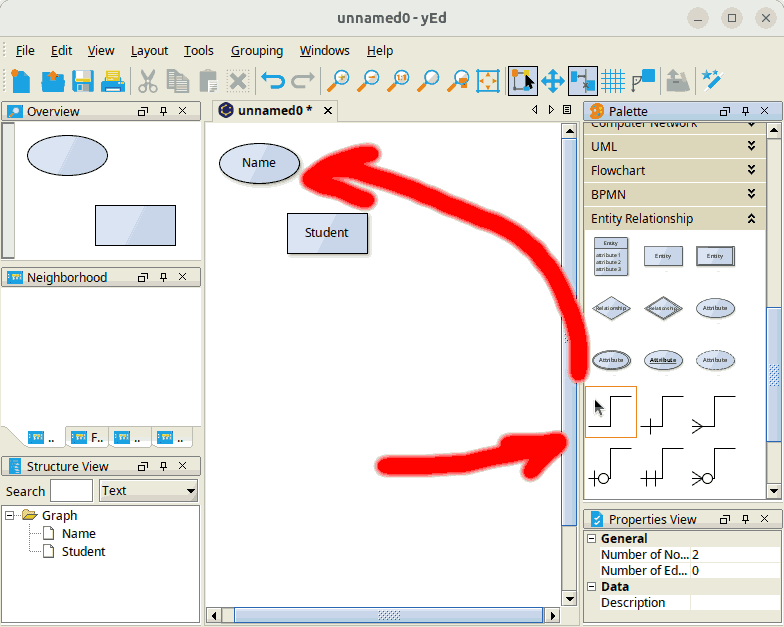
\includegraphics[width=0.48\linewidth]{\currentDir/yedErdEntitiesA10changeNameChangedToNameSelectConnection}}}%
%
\floatRowSep
%
\subfloat[][%
We drop the connection symbol onto the \emph{Name} attribute.%
\label{fig:yedErdEntitiesA11dragConnection}%
]{\tightbox{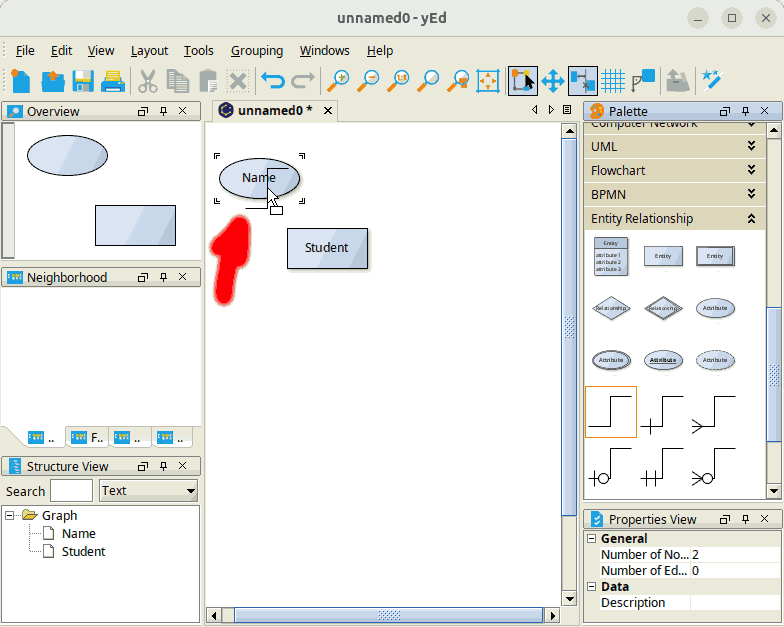
\includegraphics[width=0.48\linewidth]{\currentDir/yedErdEntitiesA11dragConnection}}}%
%
\floatSep
%
\subfloat[][%
We then click into the entity to connect the attribute \emph{Name} to the \emph{Student} entity.%
\label{fig:yedErdEntitiesA12connectToStudent}%
]{\tightbox{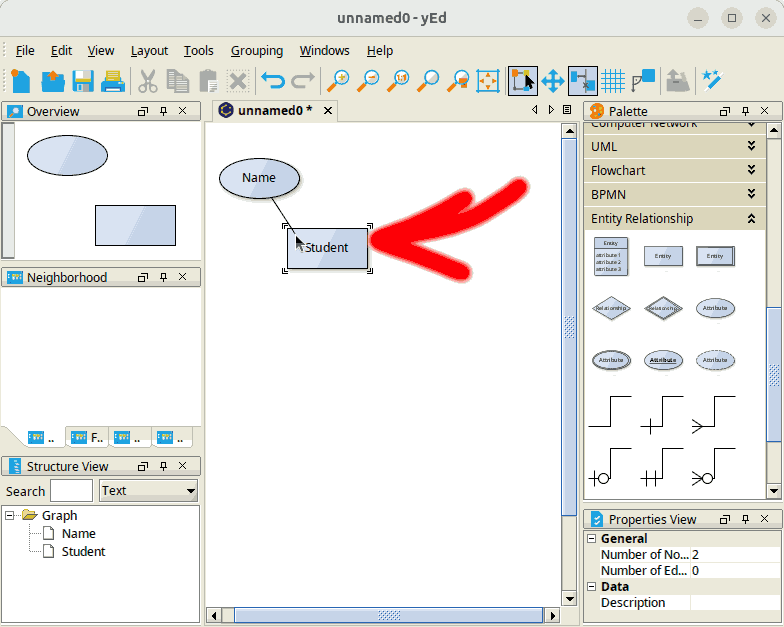
\includegraphics[width=0.48\linewidth]{\currentDir/yedErdEntitiesA12connectToStudent}}}%
%
\caption{Drawing an \pgls{ERD} with the \emph{Student} entity~(Continued).}%
\label{fig:yedErdEntitiesA:B}%
\end{figure}%
%
\begin{figure}%
\ContinuedFloat%
\centering%
%
\subfloat[][%
The \emph{Name} attribute is now connected to the \emph{Student} entity.%
\label{fig:yedErdEntitiesA13connectedToStudent}%
]{\tightbox{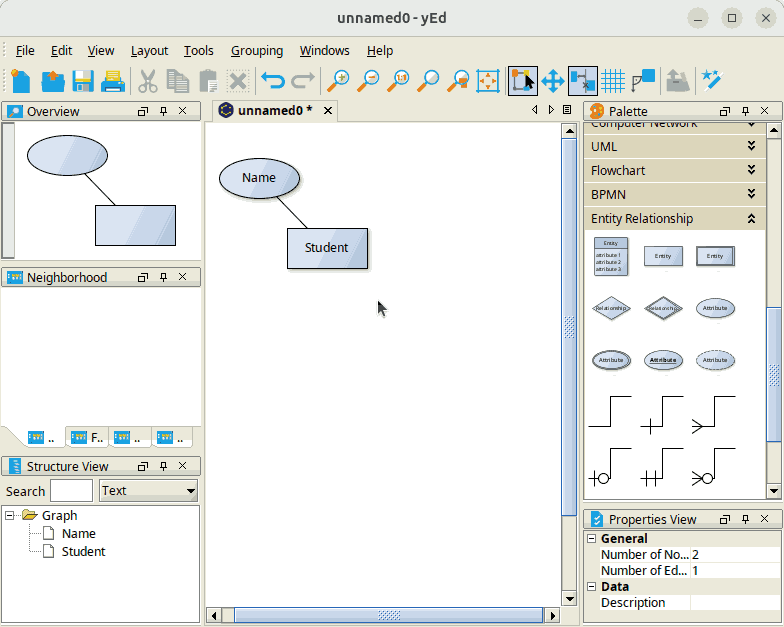
\includegraphics[width=0.48\linewidth]{\currentDir/yedErdEntitiesA13connectedToStudent}}}%
%
\floatSep%
%
\subfloat[][%
We add an attribute \emph{ID} in exactly the same way.%
\label{fig:yedErdEntitiesA14addedID}%
]{\tightbox{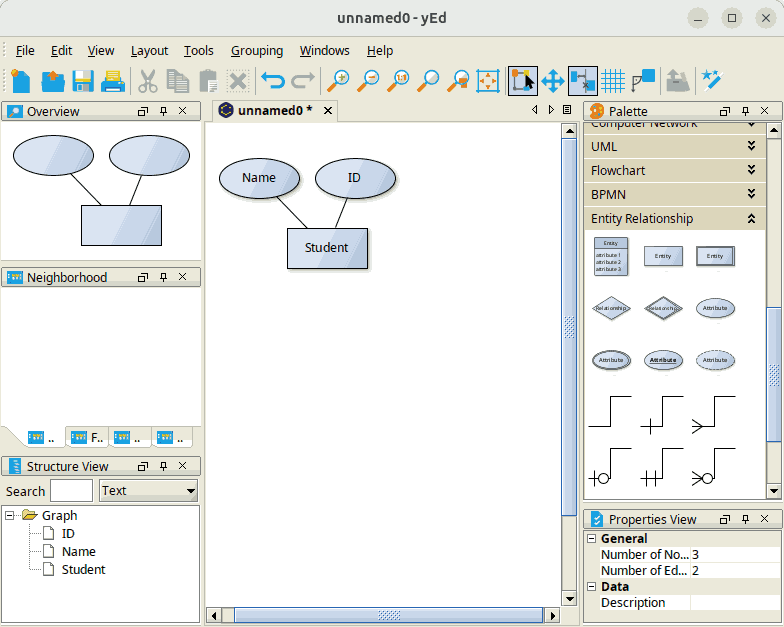
\includegraphics[width=0.48\linewidth]{\currentDir/yedErdEntitiesA14addedID}}}%
%
\floatRowSep
%
\subfloat[][%
We add several more attributes. %
Next, we click on the \menu{\underline{F}ile} menu.%
\label{fig:yedErdEntitiesA15addedAddrMobDoB}%
]{\tightbox{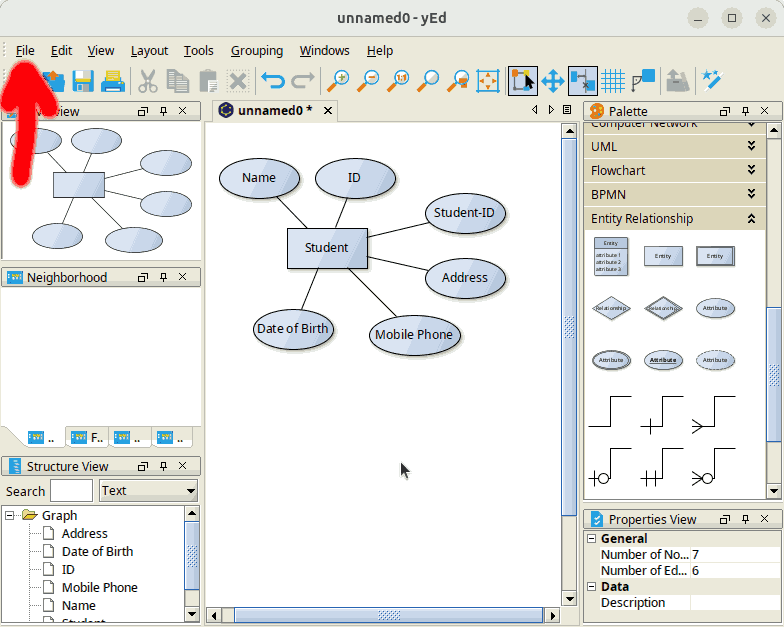
\includegraphics[width=0.48\linewidth]{\currentDir/yedErdEntitiesA15addedAddrMobDoB}}}%
%
\floatSep
%
\subfloat[][%
It is now time to save our document. %
We click on \menu{S\underline{a}ve As}.%
\label{fig:yedErdEntitiesA16saveAs}%
]{\tightbox{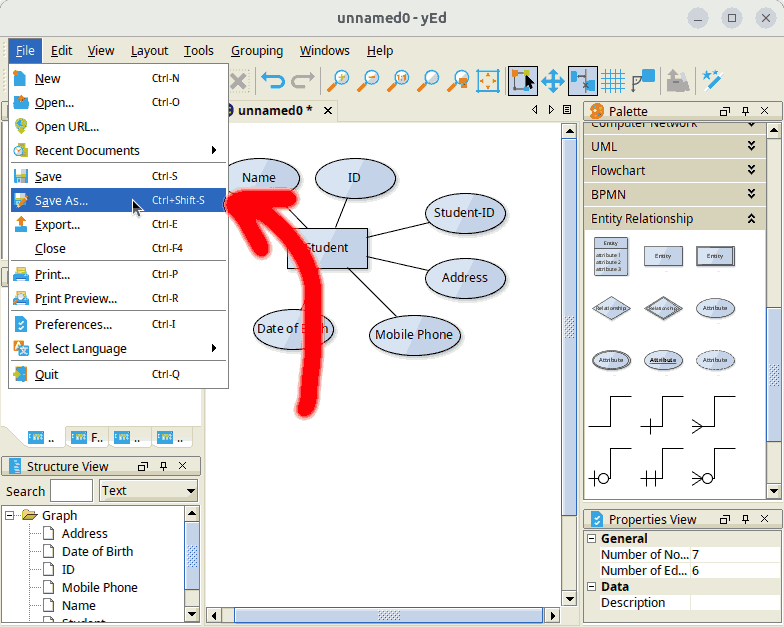
\includegraphics[width=0.48\linewidth]{\currentDir/yedErdEntitiesA16saveAs}}}%
%
\floatRowSep
%
\subfloat[][%
We save the diagram under the name \textil{erd_student_1} in the \textil{graphml} format by entering this name and clicking \menu{Save}.%
\label{fig:yedErdEntitiesA17saveAsErdStudent1}%
]{\tightbox{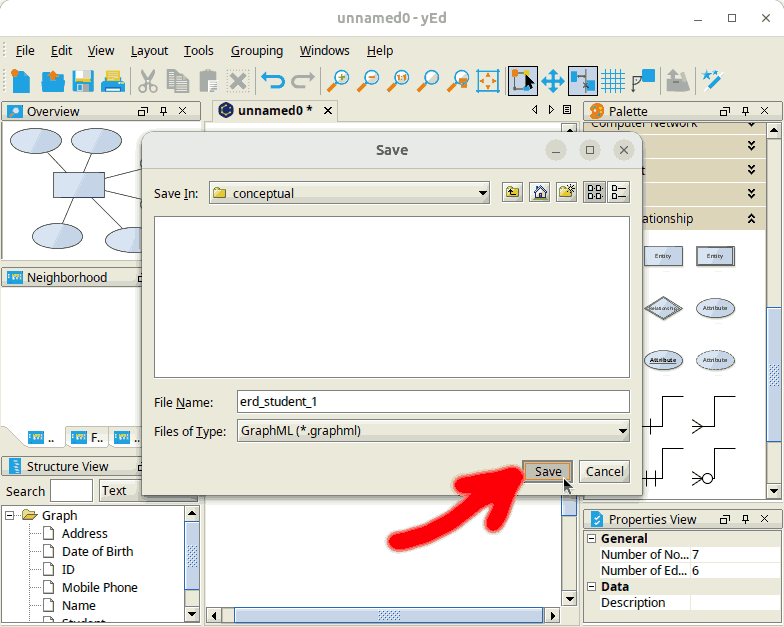
\includegraphics[width=0.48\linewidth]{\currentDir/yedErdEntitiesA17saveAsErdStudent1}}}%
%
\floatSep
%
\subfloat[][%
We can also store the diagram in a format that we can use in other documents. %
For this, we click on \menu{\underline{E}xport} in the \menu{\underline{F}ile} menu.%
\label{fig:yedErdEntitiesA18export}%
]{\tightbox{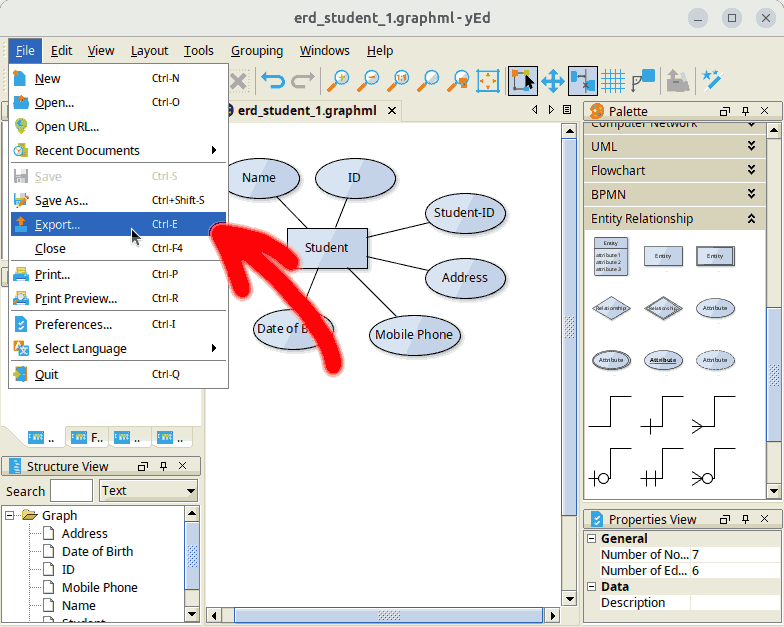
\includegraphics[width=0.48\linewidth]{\currentDir/yedErdEntitiesA18export}}}%
%
\caption{Drawing an \pgls{ERD} with the \emph{Student} entity~(Continued).}%
\label{fig:yedErdEntitiesA:C}%
\end{figure}%
%
\begin{figure}%
\ContinuedFloat%
\centering%
%
\subfloat[][%
We choose to expert in the \textil{svg} format an click \menu{Save}.%
\label{fig:yedErdEntitiesA19exportToSvg}%
]{\tightbox{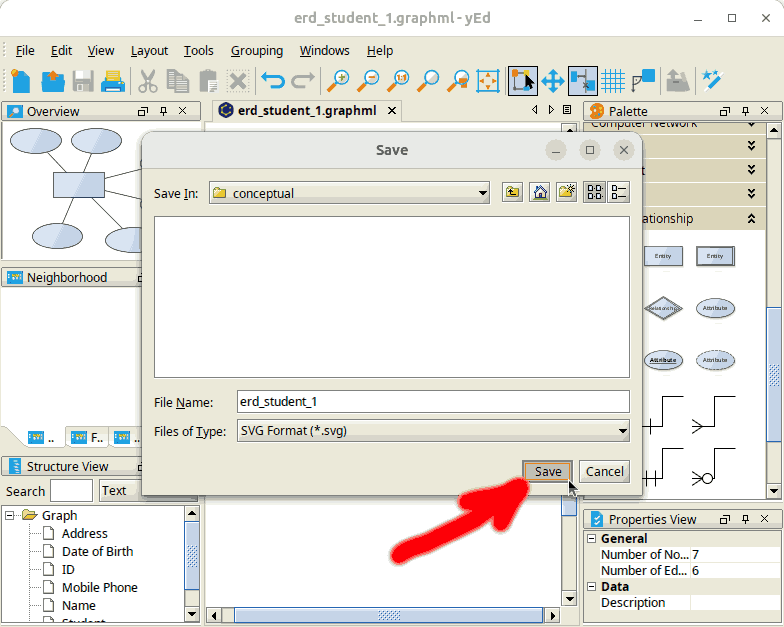
\includegraphics[width=0.48\linewidth]{\currentDir/yedErdEntitiesA19exportToSvg}}}%
%
\floatSep%
%
\subfloat[][%
We leave all settings as-is and click \menu{OK}.%
\label{fig:yedErdEntitiesA20exportToSvgDone}%
]{\tightbox{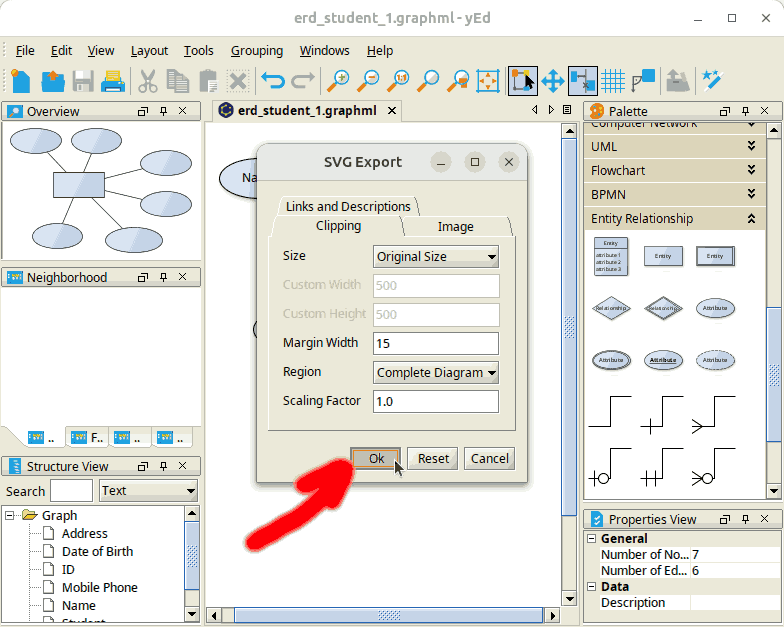
\includegraphics[width=0.48\linewidth]{\currentDir/yedErdEntitiesA20exportToSvgDone}}}%
%
\floatRowSep
%
\subfloat[][%
This produces this beautiful \pgls{ERD}.%
\label{fig:yedErdEntitiesA21erd}%
]{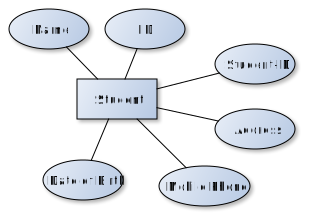
\includegraphics[width=0.6\linewidth]{\currentDir/yedErdEntitiesA21erd}}%
%
%
\caption{Drawing an \pgls{ERD} with the \emph{Student} entity~(Continued).}%
\label{fig:yedErdEntitiesA:D}%
\end{figure}%
%
\FloatBarrier%
\endhsection%
%
